%% \section{Introduction} %for journal use above \firstsection{..} instead
Word embeddings, especially cross-lingual embeddings, has been successful in multiple NLP applications such as machine translation \cite{lample2018unsupervised, artetxe2018unsupervised} and cross-lingual document classification \cite{klementiev-titov-bhattarai:2012:PAPERS}. 
But one area where there has not been very specific research is discovering the meanings of the embeddings themselves. \\

One way to efficiently convey this semantic information about embeddings is to enable an efficient interaction between humans and the visualizations of these embeddings. However, there have been a lot of problems in the current visualizations of these embeddings.
For example, there are potential problems of naively displaying the word embeddings projected onto 2D space using t-SNE \cite{t-sne}, which is not commonly used in visualizing word embeddings, such as;
\begin{itemize*}
  \item Overlap of words when zoomed out (Figure~\ref{fig:t_sne}). 
  \item A counter-intuitive features of a t-SNE visualization (e.g., ``cluster sizes mean nothing''\footnote{https://distill.pub/2016/misread-tsne/}) 
  %\item There are many other alternatives to visualize word embeddings than commonly used t-SNE (e.g., UMAP \cite{umap} or $k$-Nearest Neighbor graph), but no thorough comparison conducted. 
 %\item Which is the better way to display word embeddings to humans: k-nearest neighbor graph or t-SNE-based visualization? Does a counter-intuitive visualization using t-SNE \cite{t-sne} (e.g., ``cluster sizes mean nothing''\footnote{https://distill.pub/2016/misread-tsne/}) affect the interaction with humans? 
\end{itemize*}
%Figure~\ref{fig:graph} shows an example of $k$-nearest neighbor graph and Figure~\ref{fig:t_sne} shows an example of visualization using t-SNE. \\

\begin{figure}[htb]
 \centering
     {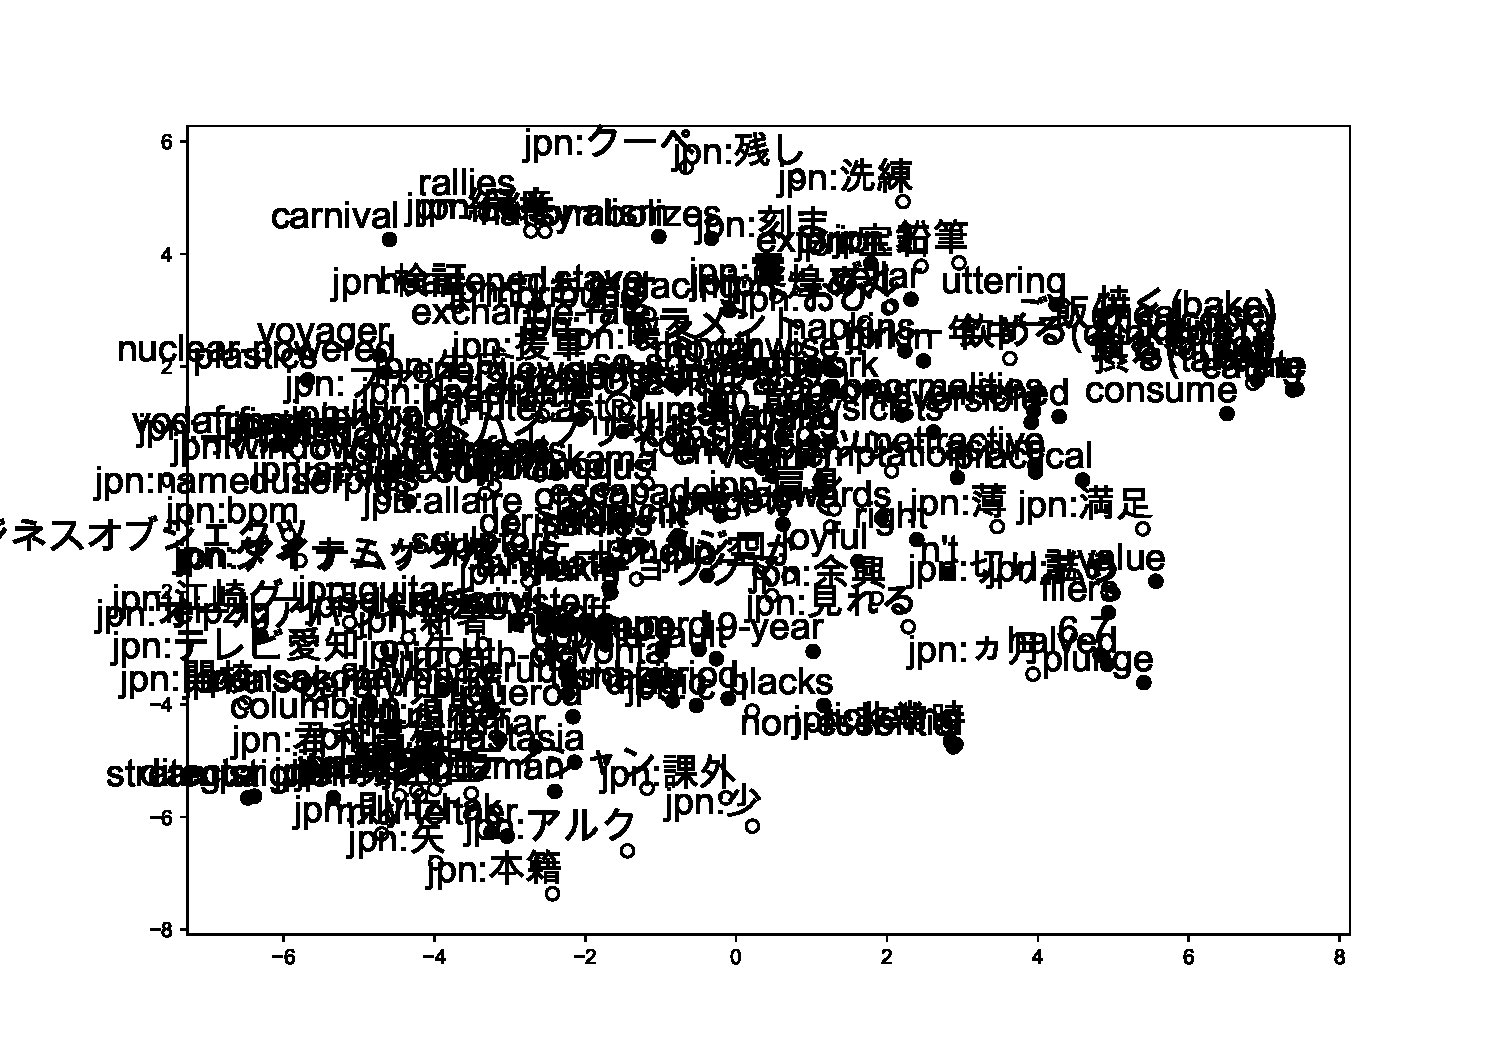
\includegraphics[width=0.78\linewidth]{figures/t_sne_en_jp_cluttered.pdf}}
    \vspace{-1ex}
     \caption{An example of a visualizaiton of word embeddings using t-SNE. Visualization of around 200 words causes clutter and makes humans hard to extract useful information. }
\label{fig:t_sne}
\end{figure}


\begin{figure}[htb]
 \centering
     {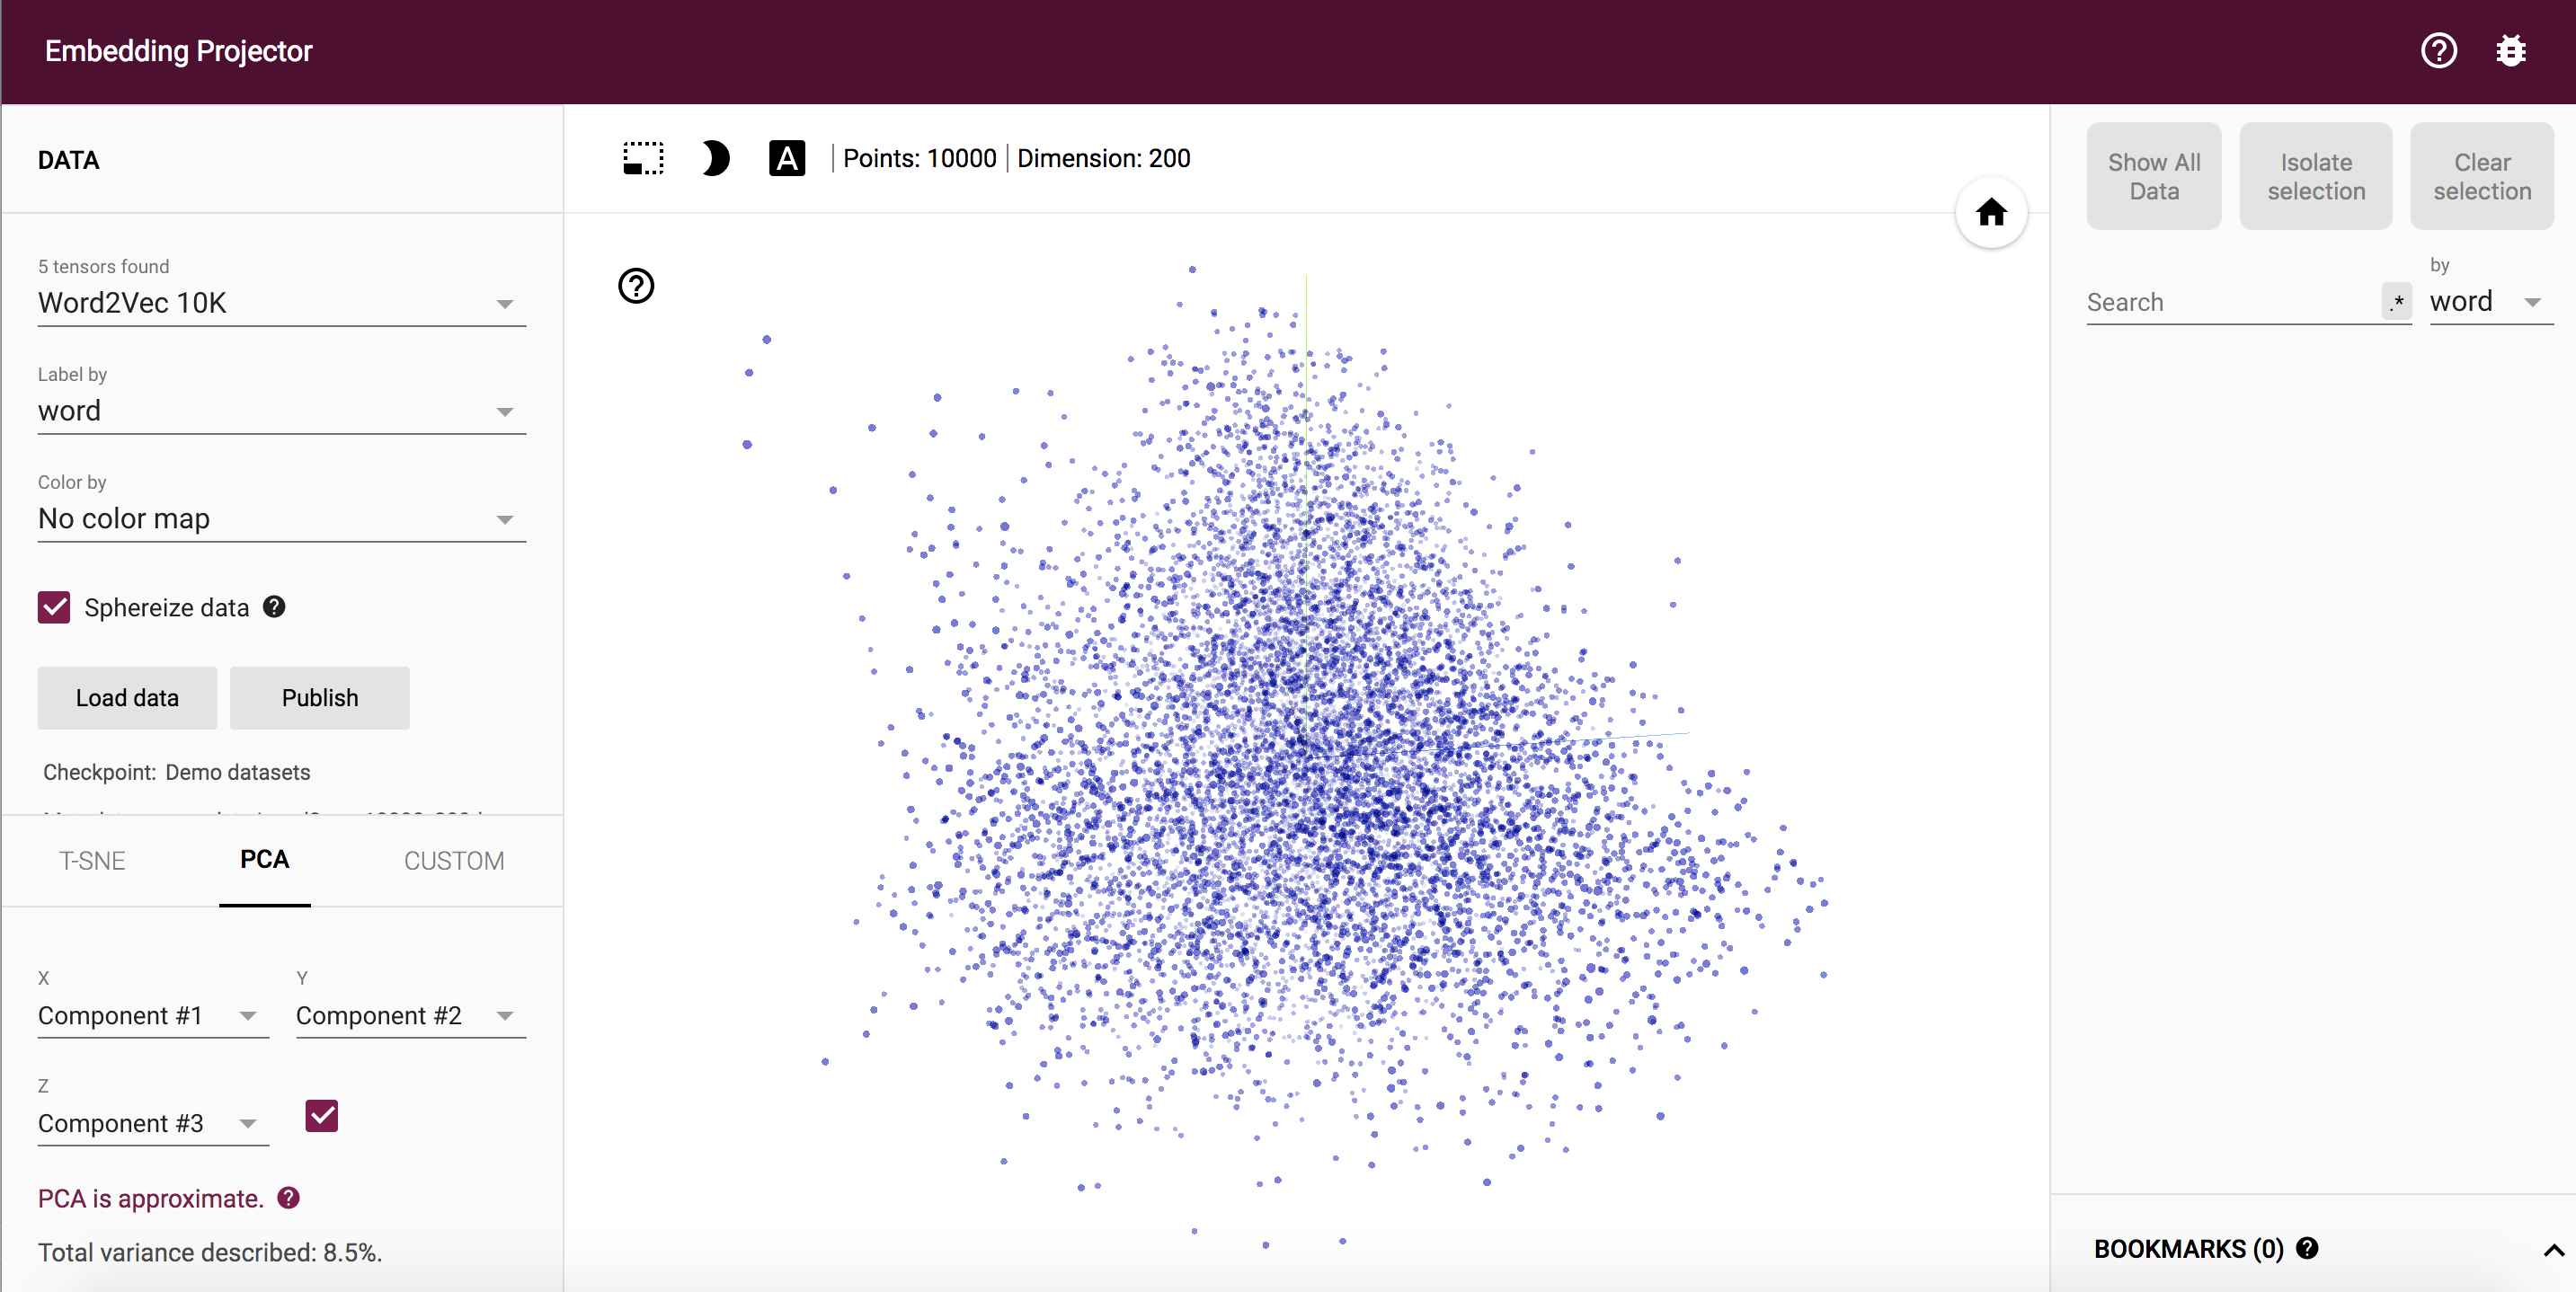
\includegraphics[width=0.78\linewidth]{figures/tensorboard.png}}
    \vspace{-1ex}
     \caption{The visualizaiton of word embeddings using Tensorboard.}
\label{fig:tensorboard}
\end{figure}



Also, many researchers decided to visualize embeddings in the 3D space, like Tensorboard (Figure~\ref{fig:tensorboard}) \cite{tensorboard_viz}, but it ends up looking like a large cluttered collection of points. A visualization like that is just useful if the goal is to just play around with the click-and-drag interaction, but in the end, there is no semantic information being conveyed. \\

The ultimate goal of any good visualization is to convey the user about everything the data represents, and not what the data is like. Therefore, we think that semantics is a crucial aspect of any good visualization. So when we decided to carry on this project, the key question we asked ourselves was - How can we represent word embeddings efficiently in a 2D design space by keeping the clutter on the design space as minimum as possible? \\

Therefore using this motivation, we carry forward this project, and accomplished the following:
\begin{itemize*}
 \item Used a 2D design space to visualize the entire word2vec embedding space.
 \item Kept the clutter minimized by having an efficient k-means clustering algorithm implemented on the cosine similarities of these word vectors.
 \item Convey the semantic information of every single cluster by annotating them with Emojis, because of their excellent way of conveying semantic information with just a single character.
\end{itemize*}


